\documentclass[twocolumn]{article}
\setlength{\parskip}{0.03cm}
\setlength{\parindent}{0.35ex}
\setlength{\columnsep}{0.5cm}
\usepackage{import}
\usepackage{scn}
\usepackage[T2A]{fontenc}
\usepackage[utf8]{inputenc}
\usepackage{indentfirst}
\usepackage[a4paper, left=2.5cm, right=1.5cm, top=2cm, bottom=2.5cm]{geometry}
\setlength{\baselineskip}{1.5em} % Пример значения
\usepackage{hyperref}
\usepackage{tcolorbox}
\usepackage{float}
\usepackage{longtable}
\usepackage{awesomebox}
\usepackage{caption}
\usepackage{multicol}
\usepackage{enumitem}
\usepackage{lipsum}
\usepackage{amsmath}
\usepackage{graphicx}
\setlist[itemize]{itemsep=0pt,topsep=0pt}


\setcounter{page}{57}
\title{лабораторная 1 дор}
\author{Аня Дорошко}
\date{Сентябрь 2024} % Изменено на русский язык

\begin{document}
\newcounter{mycounter}
\setcounter{mycounter}{8}
\newcounter{seccounter}
\setcounter{seccounter}{9}
\begin{multicols}{2}
\raggedleft
\end{multicols}


    

%\begin{minipage}
%{0.48\textwidth} %левый текст

\begin{itemize}[itemsep=0pt, topsep=0pt]
    \item\textit{     installing genetic subsystems}  
    \item\textit{   search for reusable components of ostis-systems}
    \item \textit {     installing reusable components}
    \item \textit {     configure ostis system}
\end{itemize}
 \qquad\quad:=   [configuration of the ostis system]

 \quad\quad\textrangle

   \quad Whether installing reusable components into an already created system or creating a system from scratch,
constructs are created in the ostis-system knowledge base
to denote which components are installed into the system.
Figure 7 shows an example of a construct specifying
which components are installed in an ostis system.

\quad Finding and installing an ostis-platform is necessary
because different ostis-platforms may be suitable for
different classes of tasks and components to be installed
in the generated system.

\quad By installing generic subsystems, the functionality
of the ostis-system being generated can be greatly expanded. The OSTIS Metasystem Library contains many
subsystems often used in other ostis-systems. Typical
subsystems include, for example, the subsystem for collective design of ostis-systems, natural language interface,
training subsystem, security subsystem and others.

\quad Thanks to the extensive search functionality of
reusable ostis-system components, it is possible to search
for any components according to various criteria and
combinations thereof.

\quad Customising an ostis-system implies setting parameters to specify the peculiarities of the system operation,
as well as specifying which users are administrators,
developers, experts, and users of the created ostis-system.

\quad In addition to user actions when creating an ostissystem, the ostis-system generation subsystem also registers the created ostis-system in the OSTIS Metasystem.
Thus, the OSTIS Metasystem is able to monitor and
update the status of the components of this system.                        \hfill\break


{\Roman{mycounter}}.User interface of component manager and library
of reusable components of ostis-systems
\hfill\break
\hfill\break
\quad The multi-component manager for ostis-systems has a
console interface. The component manager is connected
to sc-memory as a dynamic component, so it does
not require a restart, and you can immediately see the
installed components in a running system.
\quad Let’s look at the commands with which you can use
the component manager. Each command calls the corresponding agent. Agent-based architecture allows you
to implement any user interfaces for the component
manager of ostis-systems. Any variant of the component manager user interface creates sc-constructs in scmemory that are needed to invoke the corresponding scagent.
 
%\end{minipage} % закончился левый текст
\hfill\break
\textbf{action. Set the specifications of reusable ostis-system
components
}

$\Rightarrow $\quad agent*: \hfill\break
\begin{d}
\quad\quad [ScComponentManagerInitAgent]
\end{d}

$\Rightarrow $\quad command to initiate an action*: \hfill\break \begin{d}
\quad\quad [components init]
\end{d}
\hfill\break
\hfill\break
\textbf{action.Find specifications for reusable ostis
components
}

$\Rightarrow $\quad agent*: \hfill\break
\begin{d}
\quad\quad [ScComponentManagerSearchAgent]\hfill\break 
\end{d}
$\Rightarrow $\quad command to initiate action*: \hfill\break
\begin{d}
\quad\quad [components search]
\end{d}

$\Rightarrow $\quad possible flags*: 


\begin{itemize}
  \setlength{\itemindent}{1em}
    \item\texttt{[}\textit{author}\texttt{]} 
       \item\texttt{[}\textit{class}\texttt{]} 
       \item\texttt{[}\textit{explanation}\texttt{]} 
\end{itemize}

\hfill\break
\begin{d}
\quad When using the search command with the author flag,
you must list the system identifiers of the sc nodes that
denote the authors of the reusable component. The class
flag is used to pass the class name to the component
manager to search for components belonging to this class.
The explanation flag is used to specify a natural-language
fragment that is a substring of the component’s explanation. If multiple search flags are listed, components that
satisfy all search criteria simultaneously will be found. If
you use the component search command without flags, all
components whose specifications are downloaded will be
found.
\end{d}
\hfill\break
\hfill\break
\textbf{action. Install reusable ostis components}



$\Rightarrow $\quad agent*: \hfill\break
\begin{d}
\quad\quad [ScComponentManagerInstallAgent]\hfill\break 
\end{d}
$\Rightarrow $\quad command to initiate action*: \hfill\break
\begin{d}
\quad\quad [components install]
\end{d}

$\Rightarrow $\quad flags*: 

\begin{itemize}
  \setlength{\itemindent}{1em}
       \item\qquad\texttt{[}\textit{idtf}\texttt{]}   
\end{itemize}
\begin{flushleft}
\quad The component install command requires the mandatory idtf flag, which the component manager uses to
search by system ID for the components to be installed
and create the necessary construct to call the component
install agent.\hfill\break
\quad The interface of the reusable component library is
graphical (Fig. 8. It displays the components that are
in the library and provides access to search, browse, and
install them.
\end{flushleft}
\mbox{}
\begin{flushleft}
\quad As an example of a library of reusable components of
ostis-systems for consideration of an example of work,
let’s take the OSTIS Metasystem Library.

\quad Installation of the OSTIS Metasystem is performed
using the following command sequence.
\end{flushleft}
\begin{figure}[h]
\centering

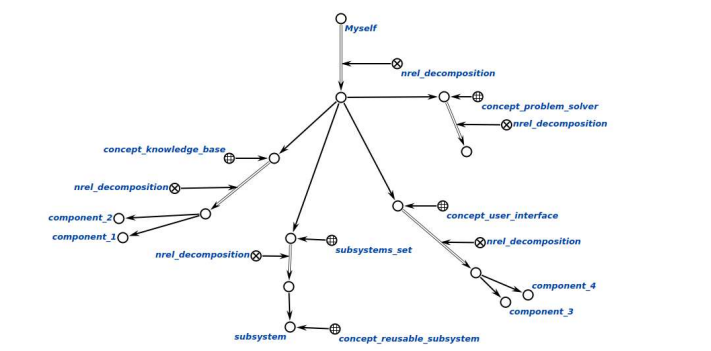
\includegraphics[width=\textwidth]{1foto.png}
    \label{fig:example}
\end{figure}
\noindent
\newpage
 \hspace{2cm}\mbox{Figure 7. Formalisation of installed components to the ostis-system}
   
\vspace{100pt}

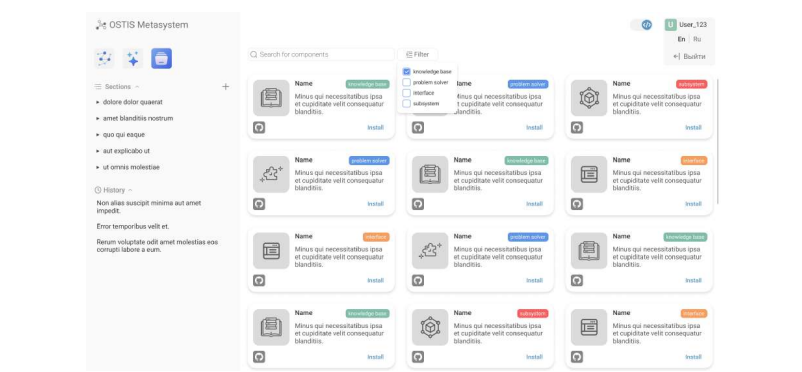
\includegraphics[width=2.3\linewidth]{foto2.png}
    \label{fig:example}
   
\noindent
 \hspace{2cm}\mbox{Figure 8. User interface of a library of reusable components of ostis-system
}

\clearpage









\renewcommand{\baselinestretch}{0.9}
\section*{\large OSTIS Metasystem}
$\Rightarrow $\quad {installation stages*}: \hfill\break 
\begin{itemize}
\item[$\langle$]\item   {Repository cloning} 
    \begin{itemize}
\item[$\Rightarrow $] \textit terminal command*: \hfill\break 
[git clone https://github.com/ostis-ai/ostis-metasystem]
 \end{itemize}   
 \end{itemize}       

\begin{itemize}
\item{Change dorectory to the project root} 
    \begin{itemize}
\item[$\Rightarrow $] \textit terminal command*: \hfill\break 
[cd ostis-metasystem]
\end{itemize}   
\end{itemize}   

\begin{itemize}
\item{OSTIS Metasystem installation} 
    \begin{itemize}
\item[$\Rightarrow $]\textit {terminal command*:} \hfill\break 
[./scripts/install\_metasystem.sh]
\end{itemize}   
\end{itemize}   


\begin{itemize}
\item{Run sc-component-manager} 
    \begin{itemize}
\item[$\Rightarrow $]\textit {terminal command*:} \hfill\break 
[./scripts/run\_sc\_component\_manager.sh]
\end{itemize}   
\end{itemize}   


\qquad\textrangle  \hfill\break 
$\Rightarrow $ \quad \textit{component installation procedure*:}





\begin{itemize}
\item\quad{Install all the reusable components\break
specifications
} 
    \begin{itemize}
\item[$\Rightarrow $]\textit {command*:} \hfill\break 
[component init]
\end{itemize}   
\end{itemize}   


\begin{itemize}
\item\quad{Reusable components searching} 
    \begin{itemize}
\item[$\Rightarrow $]\textit {command*:} \hfill\break 
[components search]
\end{itemize}   
\end{itemize}   

\begin{itemize}
\item\quad{Installation of reusable component} 
    \begin{itemize}
\item[$\Rightarrow $]\textit {command*:} \hfill\break 
\texttt [components install --  -- idtf <iden- \break
tifier>]
\end{itemize}   
\end{itemize}   

\qquad\textrangle  \hfill\break 



\textit\textbf{Creation of the core}


$\Rightarrow $\quad {stages*}: \hfill\break 
\begin{itemize}
\item[$\langle$] {\qquad Install all the reusable components \break
specifications} 
    \begin{itemize}
\item[$\Rightarrow $] \textit sc-agent*: \hfill\break 
[ScComponentManagerInitAgent]
\item[$\Rightarrow $] \textit command to call an agent*: \hfill\break 
[components init]
\item[$\Rightarrow $] \textit result*: \hfill\break 
[All the reusable components spec-\break
ifications from OSTIS Library are \break
installed.]
 \end{itemize}   
 \end{itemize}       
\begin{itemize}
\item{Search reusable user interface
components} 
    \begin{itemize}
\item[$\Rightarrow $] \textit sc-agent*: \hfill\break 
[ScComponentManagerSearchAgent]
\item[$\Rightarrow $] \textit commmand to call an agent*: \hfill\break 
[components search- -class concept-reusable-interface-component]
%\item[$\Rightarrow $] \textit result*: \hfill\break 
%[All the reusable user interface components are found.]
%\end{itemize}   
%\end{itemize}   
\hfill\break
\hfill\break


\begin{itemize}
\item\quad{Install sc-models of user interface
interpreter
} 
    \begin{itemize}
\item[$\Rightarrow $]\textit {sc-agent*:} \hfill\break 
[ScComponentManagerInstallAgent]
\end{itemize}   
\end{itemize}   

    \begin{itemize}
\item [$\Rightarrow $] \textit {commmand to call an agent*:} \hfill\break 
[ components install − idtf scweb]
\end{itemize}   
\end{itemize}   

    \begin{itemize}
\item[$\Rightarrow $]\textit {result*:
} \hfill\break 
[sc-web is intalled by specification.]
\end{itemize}   
\end{itemize} 



    \begin{itemize}
\item[$\Rightarrow $]\textit {note*:
} \hfill\break 
[If you start the web interface after
this step, only the start page will
load, because the knowledge base
is currently empty.]]
\end{itemize}   


\begin{itemize}
    \item \qquad Searching for Knowledge Base
components
\end{itemize}


  

    \begin{itemize}
\item[$\Rightarrow $]\textit {sc-agent*:} \hfill\break 
[ScComponentManagerSearchAgen]
\end{itemize}   
   

    \begin{itemize}
\item [$\Rightarrow $] \textit {commmand to call an agent*:} \hfill\break 
[ components search − − class concept-reusable-kb-component]
\end{itemize}   
 

    \begin{itemize}
\item[$\Rightarrow $]\textit {result*:
} \hfill\break 
[Received all components for
which their specification states
that they are Knowledge Base
components.]
\end{itemize}   







    \begin{itemize}
\item[$\Rightarrow $]\textit {note*:
} \hfill\break 
[If you start the web interface after
this step, only the start page will
load, because the knowledge base
is currently empty.]]
\end{itemize}   





\begin{itemize}
\item\quad{Reusable components searching} 
    \begin{itemize}
\item[$\Rightarrow $]\textit {command*:} \hfill\break 
[components search]
\end{itemize}   
\end{itemize}   

\begin{do}
\quad{Installation of reusable component} 
    \begin{itemize}
$\Rightarrow $\textit {command*:} \hfill\break 
\texttt [components install --  -- idtf <iden- \break
tifier>]
\end{itemize}   
\end{do}   



\begin{itemize}
    \item \qquad OSTIS Standard installation

components
\end{itemize}


  

    \begin{itemize}
\item[$\Rightarrow $]\textit {agent*:} \hfill\break 
[ScComponentManagerInstallAgent]
\end{itemize}   
   

    \begin{itemize}
\item [$\Rightarrow $] \textit {commmand to call an agent*:} \hfill\break 
[components install −−idtf ostis-standard]
\end{itemize}   







\subsection*{Extension of kernel functionality}

    \begin{itemize}
\item[$\Rightarrow $]\textit {stages*:} \hfill\break 
[ScComponentManagerInstallAgent]
\item {Search for all available Knowledge Base
components in the library}

\item[$\Rightarrow $]\textit {sc-agent*:} \hfill\break 
[ScComponentManagerInstallAgent]
\item {ScComponentManagerSearchAgent}


\end{itemize}   
   
\end{document}


